\documentclass[compress,red]{beamer}
\usepackage[utf8]{inputenc}
\usepackage{ucs}
\usepackage{amsmath}
\usepackage{amsfonts}
\usepackage{amssymb}
\usepackage[russian]{babel}
\usepackage{graphicx}
\usepackage{wrapfig}

\usepackage{tikz}
\usepackage{verbatim}

\usepackage{color}
\usepackage{xcolor}
\usepackage{listings}

\usepackage{caption}
\DeclareCaptionFont{white}{\color{white}}
\DeclareCaptionFormat{listing}{\colorbox{gray}{\parbox{\textwidth}{#1#2#3}}}
\captionsetup[lstlisting]{format=listing,labelfont=white,textfont=white}

\usetikzlibrary{calc,trees,positioning,arrows,chains,shapes.geometric,%
    decorations.pathreplacing,decorations.pathmorphing,shapes,%
    matrix,shapes.symbols}

\tikzset{
>=stealth',
  punktchain/.style={
    rectangle, 
    rounded corners, 
    % fill=black!10,
    draw=black, very thick,
    text width=10em, 
    minimum height=3em, 
    text centered, 
    on chain},
  line/.style={draw, thick, <-},
  element/.style={
    tape,
    top color=white,
    bottom color=blue!50!black!60!,
    minimum width=8em,
    draw=blue!40!black!90, very thick,
    text width=10em, 
    minimum height=1.5em, 
    text centered, 
    on chain},
  every join/.style={->, thick,shorten <=1pt},
  decoration={brace},
  tuborg/.style={decorate},
  tubnode/.style={midway, right=2pt},
}

\mode<presentation>

\usetheme{Warsaw}

\definecolor{Red}{rgb}{1,0,0}
\definecolor{Blue}{rgb}{0,0,1}
\definecolor{Green}{rgb}{0,1,0}
\definecolor{magenta}{rgb}{1,0,.6}
\definecolor{lightblue}{rgb}{0,.5,1}
\definecolor{lightpurple}{rgb}{.6,.4,1}
\definecolor{gold}{rgb}{.6,.5,0}
\definecolor{orange}{rgb}{1,0.4,0}
\definecolor{hotpink}{rgb}{1,0,0.5}
\definecolor{newcolor2}{rgb}{.5,.3,.5}
\definecolor{newcolor}{rgb}{0,.3,1}
\definecolor{newcolor3}{rgb}{1,0,.35}
\definecolor{darkgreen1}{rgb}{0, .35, 0}
\definecolor{darkgreen}{rgb}{0, .6, 0}
\definecolor{darkred}{rgb}{.75,0,0}

\xdefinecolor{olive}{cmyk}{0.64,0,0.95,0.4}
\xdefinecolor{purpleish}{cmyk}{0.75,0.75,0,0}

\useoutertheme[subsection=false]{smoothbars}


\title{Управляющие структуры в ruby}
\author{Информатика \\ 10-11 классы}

%\usecolortheme{dolphin}


\begin{document}
%%титульная страница
\maketitle
%% основные моменты

\section{Условия}

\subsection{Вместо введения}
\begin{frame}
  \frametitle{Вместо введения}
	\centerline{
\includegraphics[width=0.7\textwidth]{images/you_are_the_best.jpg}}
\end{frame}

\subsection{Условия}
\begin{frame}
\frametitle{Условия}
		\begin{itemize}
		\item Алгоритмы и программы зачастую имеют нелинейную структуру.
		\item В зависимости от различных параметров системы программы могут работать по-разному.
		\item Например, при логине на сайте ВКонтакте есть две возможные ситуации:
		  \begin{enumerate}
		    \item Вы вводите правильные логин и пароль и попадаете на свою страницу.
		    \item Введённая пара ``логин--пароль'' неверна, и Вас переадресовывает обратно на страницу логина
	    \end{enumerate}
	  \item Вариантов поведения может быть больше, чем два.
	  \item Такое поведение программ соответствует элементу блок--схемы ``Условие'' и структуре ``Ветвление''.
		\end{itemize}
\end{frame}

\subsection{Линейное уравнение}
\begin{frame}
  \frametitle{Блок--схема}
  Вернёмся к задаче о решении линейного уравнения.
  \begin{figure}
  \centering
  \begin{tikzpicture}[node distance=1cm, auto]  
  \tikzset{
      action/.style={rectangle,draw=black, top color=white, bottom color=yellow!50,very thick, inner sep=0.25em, minimum size=0.6em, text centered},
      input/.style={ellipse,draw=black, top color=white, bottom color=yellow!50,very thick, inner sep=0.25em, minimum size=0.6em, text centered},
      condition/.style={diamond,draw=black, top color=white, bottom color=yellow!50,very thick, inner sep=0.25em, minimum size=0.6em, text centered},
      myarrow/.style={draw},
  }
  \node[input] (item1) {Ввести $a,b,c$};  
  \node[condition, below=1em of item1] (item2) {$a == 0$};
    \node[condition, right=of item2] (item3) {$b == c$};
      \node[action, below=of item3]  (item4) {Решений нет};
      \node[action, right=of item3] (item5) {$x$ --- любое};
    \node[action, left=of item2] (item6) {$x = (c-b)/a$};

  \path[myarrow] (item1) -- (item2);   
  \path[line] (item3) -- node [near end] {да} (item2);        
  \path[line] (item6) -- node [near end] {нет} (item2);        
  \path[line] (item4) -- node [near end] {нет} (item3);        
  \path[line] (item5) -- node [near end] {да} (item3);        

  \end{tikzpicture} 
  \end{figure}
\end{frame}

\subsection{Программа}
\begin{frame}[fragile]
  \frametitle{Программа}
  \begin{lstlisting}[label=ruby1,caption=Решение линейного уравнения]
  a = 5.0
  b = 3.0
  c = -2.5
  if (a == 0)
    if (b == c)
      puts "x - any number"
    else
      puts "there is no solution"
    end
  else
    x = (c-b)/a
    puts "x = #{x}"
  end
  \end{lstlisting}
\end{frame}

\section{Разбор условий}
\subsection{Пояснения к программе}
\begin{frame}
  \frametitle{Пояснения к программе}
	\begin{itemize}
	  \item \textbf{if} ... \textbf{else} ... \textbf{end} --- оператор условия.
	  \item \textbf{if (a == 0)} означает \emph{если значение переменной a равно нулю}.
	  \item В случае, если \textbf{a} действительно равно нулю, то выполняется код, расположенный сразу после слова \textbf{if}.
	  \item Если же условие ложно (то есть, в нашем случае $a \neq 0$), то выполняется код, расположенный после \textbf{else} (\emph{else} переводится как \emph{иначе}). При ложном условии код, расположенный после \textbf{if}, просто--напросто игнорируется.
	  \item Условия могут быть вложенными друг в друга. В нашем примере после одного условия сразу же следует другое. Количество ``уровней вложенности'' не ограничено.
	  \item В конце условия ставится оператор $end$.
	\end{itemize}
\end{frame}

\subsection{Неполные условия}
\begin{frame}[fragile]
  \frametitle{Неполные условия}
	\begin{itemize}
	  \item Условия могут быть \emph{неполными} (неполное означает отсутствие ключевого слова \textbf{else}):
	\end{itemize}
	
  \begin{lstlisting}[label=ruby2,caption=Неполное условие]
  if (a == 0)
    puts "a equal to 0"
    if (b == 0)
      puts "b is equal to 0 too"
    end
  end
  \end{lstlisting}

\end{frame}

\subsection{Сокращённые условия}
\begin{frame}[fragile]
  \frametitle{Модификаторы}
  \begin{itemize}
    \item Если мы имеем неполное условие и при этом нам нужно выполнить всего одно действие, можно использовать \emph{сокращённую запись условия} (\emph{модификатор}):
  \end{itemize}
  \begin{lstlisting}[label=ruby3,caption=Модификатор]
    puts "a is equal to 0" if (a == 0)
  \end{lstlisting}
\end{frame}

\subsection{Отрицательное условие}
\begin{frame}[fragile]
  \frametitle{Отрицательный модификатор}
  \begin{itemize}
    \item А если мы хотим сделать какое-либо действие в случае, когда $a \neq 0$?
  \end{itemize}
  \begin{lstlisting}[label=ruby4,caption=Простой вариант]
    puts "a is equal to 0" if (a != 0)
  \end{lstlisting}
  \begin{itemize}
    \item Однако для лучшего понимания кода проще, когда все условия --- простые. Для этого в ruby есть \emph{ключевое слово unless}, которое можно перевести как \emph{если не}. С ним программа становится проще.
  \end{itemize}
  \begin{lstlisting}[label=ruby5,caption=Улучшенный вариант]
    puts "a is equal to 0" unless (a == 0)
  \end{lstlisting}

\end{frame}

\section{Сложные условия}

\subsection{Сложное условие}
\begin{frame}
  \frametitle{Пример}
	\centerline{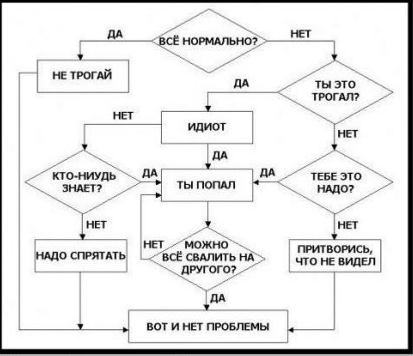
\includegraphics[width=0.7\textwidth]{images/how_to_fix_a_problem.png}}
\end{frame}

\subsection{Логические операции}
\begin{frame}[fragile]
  \frametitle{Логические операции}
  \begin{itemize}
    \item А если мы хотим одновременно проверить несколько условий? Например, если и \textbf{a}, и \textbf{b} равны нулю. Или же рассмотреть случай, когда хотя бы одна из переменных равна нулю.
    \item Для этого нужно использовать логические операции: \emph{конъюнкцию} \textbf{\&\&} и \emph{дизъюнкцию} \textbf{||}.
  \end{itemize}
  \scriptsize{
  \begin{lstlisting}[label=ruby6,caption=Конъюнкция и дизъюнкция]
    if ( (a == 0) && (b == 0) )
      puts "a and b is equal to 0"
    end
    puts "a or b is equal to 0" if ( (a == 0) || (b == 0) )
  \end{lstlisting}}

\end{frame}

\subsection{Сравнения}
\begin{frame}
  \frametitle{Сравнения}
  \begin{itemize}
    \item Что кроме \emph{проверки на равенство} можно делать в условиях?
  \end{itemize}
  \begin{center}
  \begin{table}
  \begin{tabular}{|c|l|l|}
  \hline
  Оператор & Описание & Типы переменных \\
  \hline
  == & равно & любые \\
  \hline
  != & не равно & любые \\
  \hline
  > & больше & integer, float \\
  \hline
  >= & больше либо равно & integer, float \\
  \hline
  < & меньше & integer, float \\
  \hline
  <= & меньше либо равно & integer, float \\
  \hline
  \end{tabular}
  \caption{Операторы сравнения}
  \end{table}
  \end{center}
  
\end{frame}

\section{Полное условие}
\subsection{Полное условие}
\begin{frame}[fragile]
  \frametitle{Полное условие}
  \begin{itemize}
    \item Рассмотрим реальную задачу решения квадратного уравнения.
    \item Пусть D --- дискриминант уравнения. В ней три варианта: 
      \begin{enumerate}
        \item D > 0 --- два вещественных корня,
        \item D = 0 --- один вещественный корень 2 кратности,
        \item D < 0 --- вещественных корней нет.
      \end{enumerate}
  \end{itemize}
  \scriptsize{
  \begin{lstlisting}[label=ruby7,caption=Пример полного условия]
    if (D > 0)
      puts "2 real roots"
    elsif (D == 0)
      puts "One real root"
    else
      puts "No real roots"
    end
  \end{lstlisting}}

\end{frame}

\subsection{Полное условие}
\begin{frame}[fragile]
  \frametitle{Полное условие}
  \scriptsize{
  \begin{lstlisting}[label=ruby8,caption=Схема полного условия]
    if (...)
      ...
    elsif (...)
      ...
    ...
    elsif (...)
      ...
    else
      ...
    end
  \end{lstlisting}}
  \begin{itemize}
    \item В полном условии добавляется ключевое слово \textbf{elsif}, которое переводится как \emph{иначе если}.
    \item Сначала ruby рассмотрит условие после \textbf{if}. Если оно будет ложным, он перейдёт к первому \textbf{elsif}. И так далее. Если же все условия окажутся ложными, ruby перейдёт к блоку \textbf{else}.
    \item Кстати, блок \textbf{else} не является обязательным!
  \end{itemize}

\end{frame}

\subsection{Квадратное уравнение}
\begin{frame}
  \frametitle{Квадратное уравнение}
  \begin{itemize}
    \item Итак, вернёмся к квадратному уравнению. Напишем программу, высчитывающую все корни (если таковые имеются) квадратного уравнения $ax^2+bx+c=0$.
    \item Немного упростим себе задачу, предположив, что $a \neq 0$.\footnote{Не забудьте сделать самостоятельно алгоритм без такого допущения.}
    \begin{enumerate}
      \item Вычислим дискриминант уравнения по формуле: $D = b^2 - 4ac$.
      \item Если дискриминант меньше нуля, то решений нет.
      \item Если дискриминант равен нулю, то корень --- один. Он равен: $-\cfrac{b}{2a}$.
      \item Если дискриминант больше нуля, то существует два вещественных корня:
        \begin{gather*}
          x_{1,2} = \cfrac{-b \pm \sqrt{b^2-4ac}}{2a}
        \end{gather*}
    \end{enumerate}
  \end{itemize}
  
\end{frame}

\end{document}